\chapter{Methods}
\label{method}

\TG{This chapter should have a more informative title, maybe ``Page cache simulation model''.}

\TG{Add a line of intro: ``This chapter describes our page cache simulation model and its implementation in the WRENCH framework.''}

\TG{The following comments from Review 1 should be taken into account (here and in the paper repo):

\begin{itemize}
\item In Algorithm 2 and 3, the function mm.evict has different calling parameters. What is the difference between these of overloaded methods?

\item Most of the functions called in Algorithm 2 and 3 have same functionality
as presented in the manuscript description of these algorithms but either
the function names or the order of parameters did not match in these two
algorithms. Consistency of the manuscript is key of good presentation.

\item 
Also, it would be easy to understand if the authors provide a diagram which
shows the modifications at the WRENCH design or workflow.
\end{itemize}
}

We separate our simulation model in two components, the I/O
Controller and the Memory Manager, which together simulate
file reads and writes (Figure~\ref{fig:interaction}).
To read or write a file chunk, a simulated application sends a
request to the I/O Controller. The I/O Controller interacts as needed with
the Memory Manager to free memory through flushing or eviction,
and to read or write cached data. The Memory Manager
implements these operations, simulates periodical flushing
and eviction, and reads or writes to disk when necessary.
In case the writethrough strategy is used, the I/O Controller directly writes to disk, 
cache is flushed if needed and written data is added to page cache.

\begin{figure}
       \centering
       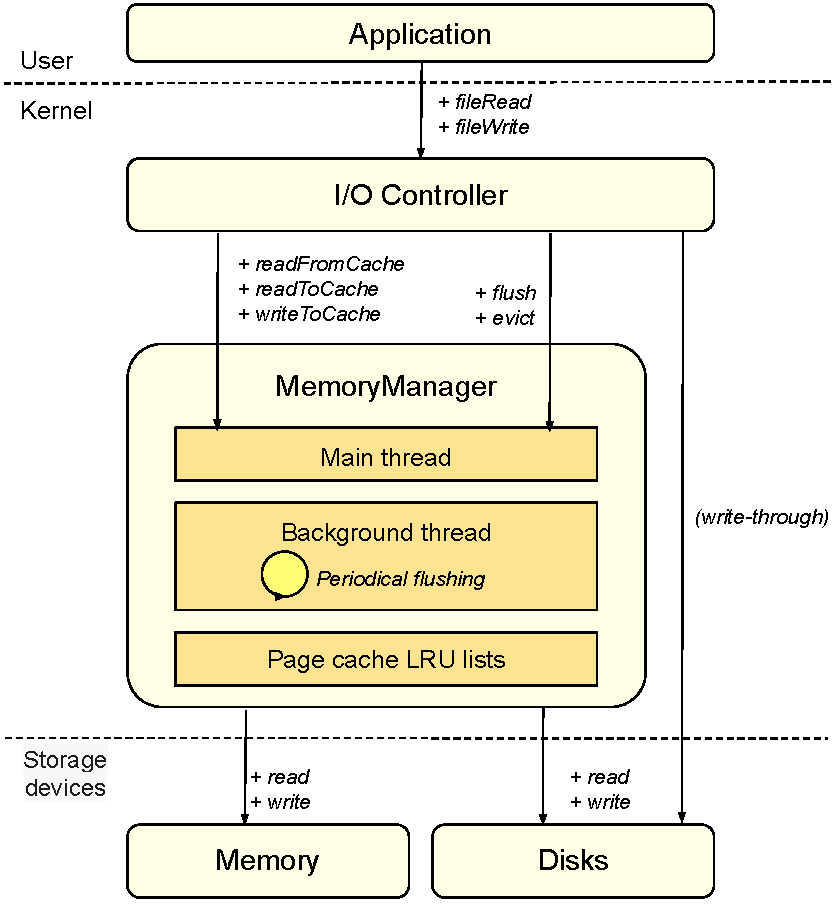
\includegraphics[width=0.7\columnwidth]{figures/interaction.pdf}
       \captionof{figure}{Overview of the page cache simulator.
       Applications send file read or write requests to the
       I/O Controller that orchestrates flushing, eviction, cache
       and disk accesses with the Memory Manager. Concurrent accesses to storage
       devices (memory and disk) are simulated using existing models.}
       \label{fig:interaction}
\end{figure}

\section{Memory Manager}

The Memory Manager simulates two parallel threads: the main one
implements flushing, eviction, and cached I/Os synchronously, whereas
the second one, which operates in the background, periodically searches for
expired dirty data in LRU lists and flushes this data to disk. We
use existing storage simulation models~\cite{lebre2015} to simulate disk and
memory, characterized by their storage capacity, read and write
bandwidths, and latency. These models account for
bandwidth sharing between concurrent memory or disk accesses.

\subsection{Page cache LRU lists}

In the Linux kernel, page cache LRU lists contain file pages. However,
due to the large number of file pages, simulating lists of pages
induces substantial overhead.
Therefore, we introduce the concept of a data block as a unit to represent data
cached in memory. A data block is a subset of file pages stored in
page cache that were accessed in the same I/O operation.
A data block stores the file name, block size, last access
time, a dirty flag that represents whether the data is clean (0)
or dirty (1), and an entry (creation) time.
Blocks can have different sizes and a given file can have multiple
data blocks in page cache. In addition, a data block can be split into an
arbitrary number of smaller blocks.

\begin{figure}
       \centering
       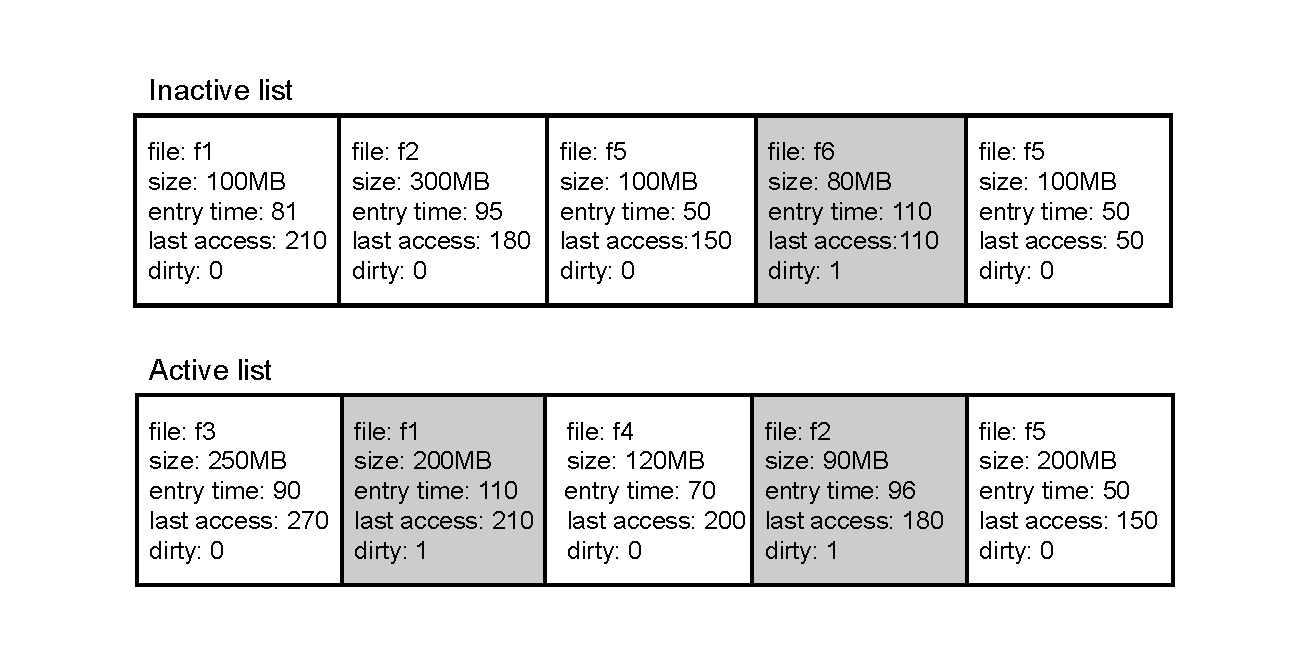
\includegraphics[width=0.8\columnwidth]{figures/lru_lists.pdf}
       \caption{Model of page cache LRU lists with data blocks.}
       \label{fig:lrulist}
\end{figure}

We model page cache LRU lists as
two lists of data blocks, an active list and an inactive list, both ordered by
last access time (earliest first, Figure~\ref{fig:lrulist}).
As in the kernel, our simulator limits the size of the active list to
twice the size of the inactive list, by moving least recently
used data blocks from the active list to the inactive list~\cite{gorman2004understanding, linuxdev3rd2010}.

At any given time, a file can be partially cached, completely cached,
or not cached at all. A cached data block can only reside in one of two
LRU lists. The first time they are accessed, blocks are
added to the inactive list. On subsequent accesses, blocks of the
inactive list are moved to the top of the active list. Blocks
written to cache are marked dirty until flushed.

\subsection{Reads and writes}

Our simulation model supports chunk-by-chunk file accesses
with a user-defined chunk size. However, for simplicity, we assume that file pages are
accessed in a round-robin fashion rather than fully randomly.
Therefore, when a file is read, cached data is read only after all uncached data was read, and data from the inactive list is read
before data from the active list
(data reads occur from left to right in Figure~\ref{fig:read_order}).
When a chunk of \emph{uncached} data is read, a new clean block is created
and appended to the inactive list.
When a chunk of \emph{cached} data is read, one or more existing data blocks in the LRU lists are accessed.
If these blocks are clean, we merge them together, update the access time and size of the resulting block,
and append it to the active list.
If the blocks are dirty, we move them independently to the active list, to preserve their entry time.
Because the chunk and block sizes may be different, there are situations
where a block is not entirely read.
In this case, the block is split in two smaller blocks and one of them is re-accessed.
% From Tristan: not sure where to put this nor if it's necessary:
% , in which chunks are read/written
% until file is entirely read/written.

\begin{figure}
       \centering
       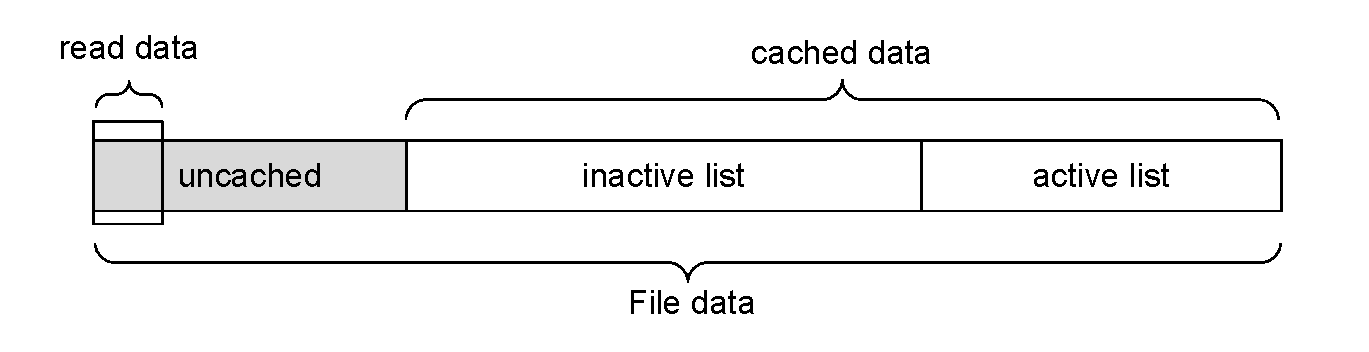
\includegraphics[width=0.8\columnwidth]{figures/read_order.pdf}
       \caption{File data read order. Data is read from left to right: uncached data
       is read first, followed by data from the inactive list, and finally data from the active list. }
       \label{fig:read_order}
\end{figure}

For file writes, we assume that all data to be written is
uncached. Thus, each time a chunk is written, we create a block of dirty data
and append it to the inactive list.

\subsection{Flushing and eviction}

The main simulated thread in the Memory Manager can flush or evict data from the
memory cache. The data flushing simulation
function takes the amount of data to flush as parameter. While
this amount is not reached and dirty
blocks remain in cache, this function traverses the sorted
inactive list, then the sorted active list, and writes the
least recently used dirty block to disk, having set its dirty
flag to 0. In case the amount of data to flush requires that a
block be partially flushed, the block is split in two blocks,
one that is flushed and one that remains dirty. The time needed
to flush data to disk is simulated by the storage model.

The cache eviction simulation also runs in
the main thread. It frees up the page cache by traversing and deleting
least recently used clean data blocks in the inactive list.
The amount of data to evict is passed as a parameter and data blocks are deleted
from the inactive list until the evicted data reaches the required amount,
or until there is no clean block left in the list.
If the last evicted block does not have to be entirely evicted, the block is split in two blocks,
and only one of them is evicted.
The overhead of the cache eviction algorithm is not part of the simulated time
since cache eviction time is negligible in real systems. % \tristan{a reference would be welcome}.

\begin{algorithm}[H]
\caption{Periodical flush simulation in Memory Manager}
\label{alg:pdflush}
    \small
    \begin{algorithmic}[1]
        \Input
            \Desc{in}{page cache inactive list}
            \Desc{ac}{page cache active list}
            \Desc{t}{predefined flushing time interval}
            \Desc{exp}{predefined expiration time}
            \Desc{sm}{storage simulation model}
           \EndInput
           \While{host is on}
            \State blocks = expired\_blocks(exp, in) + expired\_blocks(exp, ac)
            \State flushing\_time = 0
            \For{blk in blocks} 
              \State blk.dirty = 0 
              \State flushing\_time = flushing\_time + sm.write(blocks)
            \EndFor
            \If{flushing\_time $<$ t}
                \State sleep(t - flushing\_time)
            \EndIf  
        \EndWhile
    \end{algorithmic}
\end{algorithm}

Periodical flushing is simulated in the Memory Manager
background thread. As in the Linux kernel, a dirty block
in our model is considered expired if
the duration since its entry time is longer than a
predefined expiration time.
Periodical flushing is simulated as an infinite loop in which
the Memory Manager searches for dirty blocks and flushes them to disk (Algorithm~\ref{alg:pdflush}).
% From Tristan: the algorithm is quite straightforward, I don't think this is
% necessary
% In each repetition, Memory Manager finds expired dirty blocks in two
% page cache LRU lists (line 8), simulates writes of data of these blocks
% to disk (line 9), and mark them as clean (line 10).
% If the flushing time does not exceed our time interval, the thread is put
% to sleep for the remaining time (lines 11-13).
% Then based on the state of the host at current simulated time,
% the algorithm continues or finishes the loop.
Because periodical flushing is simulated as a background thread, it can happen concurrently
with disk I/O initiated by the main thread. This is taken into account by the
storage model and reflected in simulated I/O time.
\section{I/O Controller}

As mentioned previously, our model reads and writes file chunks in a
round-robin fashion. To read a file chunk, simulated applications send
chunk read requests to the I/O Controller which processes them using
Algorithm~\ref{alg:read}. First, we calculate the amount of uncached
data that needs to be read from disk, and the remaining amount is read
from cache (line 7-8). The amount of memory required to read the chunk
is calculated, corresponding to a copy of the chunk in anonymous memory
and a copy of the chunk in cache (line 9).
If there is not enough available memory, the Memory Manager is called
to flush dirty data (line 10). If necessary, flushing is complemented by
eviction (line 11). Note that, when called with negative arguments, functions
\texttt{flush} and \texttt{evict} simply return and do not do anything. 
Then,if the block requires uncached data, the memory manager is called 
to read data from disk and to add this data to cache (line 14).
If cached data needs to be read, the Memory Manager is called to simulate
a cache read  and update the corresponding data blocks accordingly (line 17).
Finally, the memory manager is called to deallocate the amount of anonymous 
memory used by the application (line 19).

\begin{algorithm}[H]
\caption{File chunk read simulation in I/O Controller}
\label{alg:read}
    \small
    \begin{algorithmic}[1]
        \Input
            \Desc{cs}{chunk size}
            \Desc{fn}{file name}
            \Desc{fs}{file size (assumed to fit in memory)}
            \Desc{mm}{MemoryManager object}
            \Desc{sm}{storage simulation model}
           \EndInput
           \State disk\_read = min(cs, fs - mm.cached(fn)) \Comment{To be read from disk}
           \State cache\_read = cs - disk\_read \Comment{To be read from cache}
           \State required\_mem = cs + disk\_read
           \State mm.flush(required\_mem - mm.free\_mem - mm.evictable)
           \State mm.evict(required\_mem - mm.free\_mem)
           \If {disk\_read $>$ 0}  \Comment{Read uncached data}
           \State sm.read(disk\_read)
           \State mm.add\_to\_cache(disk\_read, fn)
           \EndIf
           \If {cache\_read $>$ 0} \Comment{Read cached}
           \State mm.cache\_read(cache\_read)
        \EndIf
        \State mm.use\_anonymous\_mem(cs)
    \end{algorithmic}
\end{algorithm}

Algorithm~\ref{alg:write} describes our simulation of chunk writes in
the I/O Controller.
% Data is written to cache until the amount of dirty data in the cache
% exceeds the dirty ratio times the amount of available memory. Data is then written to disk.
Our algorithm initially checks the  amount of dirty data that
can be written given the dirty ratio (line 5).
If this amount is greater than 0, the Memory Manager is requested to evict
data from cache if necessary (line 7).
After eviction, the amount of data that can be written to
page cache is calculated (line 8), and a cache write is simulated (line 9).
If the dirty threshold is reached and there is still data to write,
the remaining data is written to cache in a loop
where we repeatedly flush and evict from the cache (line 12-18).

\begin{algorithm}[H]
\caption{File chunk write simulation in I/O Controller}
\label{alg:write}
    \small
    \begin{algorithmic}[1]
        \Input
            \Desc{cs}{chunk size}
            \Desc{fn}{file name}
            \Desc{mm}{MemoryManager object}
           \EndInput
        \State remain\_dirty = dirty\_ratio * mm.avail\_mem - mm.dirty
        \If {remain\_dirty $>$ 0} \Comment{Write to memory}
            \State mm.evict(min(cs, remain\_dirty) - mm.free\_mem)
            \State mem\_amt = min(cs, mm.free\_mem)
            \State mm.write\_to\_cache( mem\_amt, fn)
        \EndIf
        \State remaining = cs - mem\_amt
        \While {remaining $>$ 0}  \Comment{Flush to disk, then write to cache}
            \State mm.flush(cs - mem\_amt)
            \State mm.evict(cs - mem\_amt  - mm.free\_mem)
            \State to\_cache = min(remaining, mm.free\_mem)
            \State mm.write\_to\_cache(to\_cache, fn)
            \State remaining = remaining - to\_cache
        \EndWhile

    \end{algorithmic}
\end{algorithm}

The above model describes page cache in writeback
mode. Our model also includes a write function in writethrough mode,
which simply simulates a disk write with the amount of data passed in,
then evicts cache if needed and adds the written data to the cache.
\section{Implementation}

We first created a standalone prototype
simulator to evaluate the accuracy and correctness of our
model in a simple scenario before integrating it in the more complex
\wrench framework.
The prototype uses the following basic storage model for
both memory and disk:
\begin{align*}
    & t_{r} = D / b_r \\
    & t_{w} = D / b_w\
\end{align*}

where:
\begin{itemize}
    \item $t_{r}$ is the data read time
    \item $t_{w}$ is the data write time
    \item $D$ is the amount of data to read or write
    \item $b_r$ is the read bandwidth of the device
    \item $b_w$ is the write bandwidth of the device
\end{itemize}

This prototype does not simulate  bandwidth sharing and thus does not support
concurrency: it is limited to single-threaded applications running on systems
with a single-core CPU. We used this prototype for a first validation of our simulation
model against a real sequential application running on a real system.
The Python 3.7 source code is available at
\url{https://github.com/big-data-lab-team/paper-io-simulation/tree/master/exp/pysim}.

We also implemented our model as part of \wrench, enhancing its
internal implementation and APIs with a page cache abstraction,
and allowing users to activate the feature via a command-line
argument. We used SimGrid's locking mechanism to handle
concurrent accesses to page cache LRU lists by the two Memory
Manager threads. For the experiments, we used
\wrench 1.6 at commit
\href{https://github.com/wrench-project/wrench/tree/67185374330d2c4bf274fce222c937e838df5b03}{6718537433},
which uses \simgrid 3.25, available at
\url{https://framagit.org/simgrid/simgrid}. Our implementation
is now part of \wrench's master branch and will be available to
users with the upcoming 1.8 release. \wrench provides a full \simgrid-based simulation 
environment that supports, among other features, concurrent accesses to storage devices, 
applications distributed on multiple hosts, network transfers, 
and multi-threading. 

